% ================================================================
%  CHAPTER 5 - RELEASE 2: GOVERNANCE & SECURITY HARDENING
% ================================================================
\chapter{Release 2: Governance \& Security Hardening}

\section{Introduction}

With the foundational security perimeter and core AI orchestration engine established in Release 1, the platform successfully authenticates and routes AI requests. However, enterprise adoption requires strict data governance, cost control, and advanced threat mitigation. The purpose of Release 2 is to enforce centralized governance policies and harden the platform against AI-specific vulnerabilities. This release introduces dynamic policy evaluation, tenant-level token quotas, and active data sanitization. The work included in this release spans two sprints.

% ──────────────────────────────────────────────────────────────────
\section{Release 2 Plan}
% ──────────────────────────────────────────────────────────────────

The development plan for Release 2 focuses on establishing robust guardrails for AI usage, structured into two consecutive sprints:

\begin{enumerate}
    \item \textbf{Sprint 3: Governance \& Policy Engine} - Implements Open Policy Agent (OPA) for evaluating dynamic data sensitivity rules and integrates Redis to enforce per-tenant daily token quotas, preventing cost overruns.
    
    \item \textbf{Sprint 4: Security Hardening} - Focuses on data sovereignty and AI-specific threat mitigation. It introduces PostgreSQL Row-Level Security (RLS) for absolute tenant isolation, HashiCorp Vault for secrets management, and Microsoft Presidio for real-time Personally Identifiable Information (PII) redaction.
\end{enumerate}

By focusing on these areas, we ensure that AI interactions comply with enterprise data policies and that sensitive information is strictly protected from exposure.

% ──────────────────────────────────────────────────────────────────
\section{Release 2 Backlog}
% ──────────────────────────────────────────────────────────────────

The following table outlines the backlog items identified for Release 2, covering both Sprint 3 and Sprint 4.

\begin{table}[H]
\centering
\renewcommand{\arraystretch}{1.3}
\footnotesize
\begin{tabularx}{\textwidth}{| >{\raggedright\arraybackslash}p{3.5cm} | c | >{\raggedright\arraybackslash}X | c |}
\hline
\rowcolor{rowgray}
\textbf{Feature} & \textbf{ID} & \textbf{User Stories} & \textbf{Priority} \\
\hline
Policy Definitions & 20 & As an admin, I want YAML-driven governance policies. & + + + \\
\hline
Policy Engine & 21 & As a developer, I want a policy evaluation engine. & + + + \\
\hline
Policy Auditing & 22 & As a developer, I want policy audit logs. & + + \\
\hline
Token Quotas & 23 & As an admin, I want configurable daily token quotas. & + + + \\
\hline
Quota Counters & 24 & As a developer, I want Redis-backed quota counters. & + + + \\
\hline
Tenant Isolation & 25 & As a security engineer, I want PostgreSQL RLS. & + + + \\
\hline
Secrets Management & 26 & As an operator, I want Vault managing secrets. & + + + \\
\hline
Usage Tracking & 27 & As a developer, I want a usage tracking table. & + + \\
\hline
Database Migrations & 28 & As a developer, I want automated database migrations. & + + \\
\hline
Injection Detection & 29 & As a security engineer, I want prompt injection detection. & + + + \\
\hline
Security Patterns & 30 & As a security engineer, I want database-driven security patterns. & + + \\
\hline
PII Detection & 31 & As a developer, I want PII detection (SSN, IBAN, credit card). & + + + \\
\hline
Sensitivity Escalation & 32 & As a developer, I want auto sensitivity escalation on PII. & + + \\
\hline
Data Redaction & 33 & As a developer, I want output PII redaction. & + + + \\
\hline
\end{tabularx}
\caption{Release 2 Backlog}
\label{tab:release2_backlog}
\end{table}


% ══════════════════════════════════════════════════════════════════
%  SPRINT 3: GOVERNANCE & POLICY ENGINE
% ══════════════════════════════════════════════════════════════════
\section{Sprint 3: Governance \& Policy Engine}

The goal of this sprint is to introduce dynamic policy evaluation and cost control mechanisms. By leveraging Open Policy Agent (OPA) and Redis, the platform ensures that AI requests comply with organizational data sensitivity constraints and adhere to allocated budgets.

\begin{table}[H]
\centering
\renewcommand{\arraystretch}{1.3}
\footnotesize
\begin{tabularx}{\textwidth}{| >{\raggedright\arraybackslash}p{3.5cm} | c | >{\raggedright\arraybackslash}X | c |}
\hline
\rowcolor{rowgray}
\textbf{Feature} & \textbf{ID} & \textbf{User Stories} & \textbf{Priority} \\
\hline
Policy Definitions & 20 & As an admin, I want YAML-driven governance policies. & + + + \\
\hline
Policy Engine & 21 & As a developer, I want a policy evaluation engine. & + + + \\
\hline
Policy Auditing & 22 & As a developer, I want policy audit logs. & + + \\
\hline
Token Quotas & 23 & As an admin, I want configurable daily token quotas. & + + + \\
\hline
Quota Counters & 24 & As a developer, I want Redis-backed quota counters. & + + + \\
\hline
\end{tabularx}
\caption{Sprint 3 Backlog}
\label{tab:sprint3_backlog}
\end{table}

\subsection{Software Design}

\subsubsection{Dynamic View: Governance Policy Evaluation Sequence}

Governance and Real-Time Policy Enforcement rely on the Open Policy Agent (OPA). The orchestrator dynamically evaluates custom governance rules covering data sensitivity constraints, environmental isolation, and budget consumption before authorizing any downstream routing. Additionally, Redis is used for ultra-low latency, atomic tenant quota tracking, shielding the platform from resource exhaustion.

\begin{figure}[H]
    \centering
    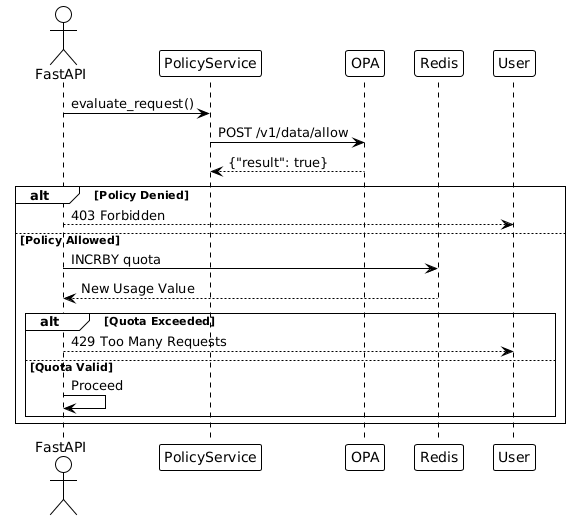
\includegraphics[width=0.85\textwidth]{images/sprint3_sequence.png}
    \caption{Governance Policy and Quota Evaluation Sequence}
    \label{fig:sprint3_sequence}
\end{figure}

The sequence diagram illustrates the policy enforcement flow:
\begin{enumerate}
    \item The FastAPI backend receives an authenticated request.
    \item Before processing the AI intent, the backend queries the Redis instance to verify the tenant's daily token quota.
    \item If the quota is exceeded, the request is immediately rejected to prevent cost overruns.
    \item If the quota is valid, the backend queries the OPA engine, passing the tenant context, request sensitivity, and requested service.
    \item OPA evaluates the declarative Rego policies and returns an authoritative decision (Allow/Deny).
    \item The backend enforces the decision, proceeding with orchestration only if authorized, and logging the outcome in the audit ledger.
\end{enumerate}

\subsection{Showcase}
\label{subsec:sprint3_showcase}

The following figures demonstrate the implementation of declarative governance and token-based cost controls.

\begin{figure}[H]
    \centering
    \includegraphics[width=0.85\textwidth]{images/token_usage_ui.png}
    \caption{Real-time token quota tracking and consumption monitoring for the 'acme-corp' tenant.}
    \label{fig:token_usage}
\end{figure}

\begin{figure}[H]
    \centering
    \includegraphics[width=0.85\textwidth]{images/governance_rules.png}
    \caption{Declarative governance policies defined in the Admin Portal and synced to OPA.}
    \label{fig:governance_rules}
\end{figure}

\begin{figure}[H]
    \centering
    \includegraphics[width=0.85\textwidth]{images/policy_audit_db.png}
    \caption{Database records showing the enforcement of sensitivity-based AI governance rules.}
    \label{fig:policy_audit}
\end{figure}


% ══════════════════════════════════════════════════════════════════
%  SPRINT 4: SECURITY HARDENING
% ══════════════════════════════════════════════════════════════════
\section{Sprint 4: Security Hardening}

With governance in place, Sprint 4 focuses on absolute data sovereignty and mitigating AI-specific vulnerabilities, such as prompt injection and data exfiltration. The system introduces PostgreSQL Row-Level Security (RLS) and integrates Microsoft Presidio for proactive threat mitigation and data sanitization.

\begin{table}[H]
\centering
\renewcommand{\arraystretch}{1.3}
\footnotesize
\begin{tabularx}{\textwidth}{| >{\raggedright\arraybackslash}p{3.5cm} | c | >{\raggedright\arraybackslash}X | c |}
\hline
\rowcolor{rowgray}
\textbf{Feature} & \textbf{ID} & \textbf{User Stories} & \textbf{Priority} \\
\hline
Tenant Isolation & 25 & As a security engineer, I want PostgreSQL RLS. & + + + \\
\hline
Secrets Management & 26 & As an operator, I want Vault managing secrets. & + + + \\
\hline
Usage Tracking & 27 & As a developer, I want a usage tracking table. & + + \\
\hline
Database Migrations & 28 & As a developer, I want automated database migrations. & + + \\
\hline
Injection Detection & 29 & As a security engineer, I want prompt injection detection. & + + + \\
\hline
Security Patterns & 30 & As a security engineer, I want database-driven security patterns. & + + \\
\hline
PII Detection & 31 & As a developer, I want PII detection (SSN, IBAN, credit card). & + + + \\
\hline
Sensitivity Escalation & 32 & As a developer, I want auto sensitivity escalation on PII. & + + \\
\hline
Data Redaction & 33 & As a developer, I want output PII redaction. & + + + \\
\hline
\end{tabularx}
\caption{Sprint 4 Backlog}
\label{tab:sprint4_backlog}
\end{table}

\subsection{Database Design}

\subsubsection{Row-Level Security (RLS)}

Traditional multi-tenant architectures often rely on Application-Level Filtering (e.g., appending \texttt{WHERE tenant\_id = X} to database queries). This approach is highly susceptible to human error and data leaks. To guarantee absolute data sovereignty, the platform implements Row-Level Security (RLS) directly at the PostgreSQL kernel level. During request execution, the authenticated \texttt{tenant\_id} extracted from the JWT is passed as a session variable to the database engine. RLS policies dynamically restrict the visibility of rows at the lowest storage tier, ensuring deterministic tenant isolation regardless of how the application layer attempts to query the data.

\subsection{Software Design}

\subsubsection{Dynamic View: Threat Mitigation and PII Redaction}

Proactive threat mitigation requires inspecting both the inbound user prompt and the outbound AI response.

\begin{figure}[H]
    \centering
    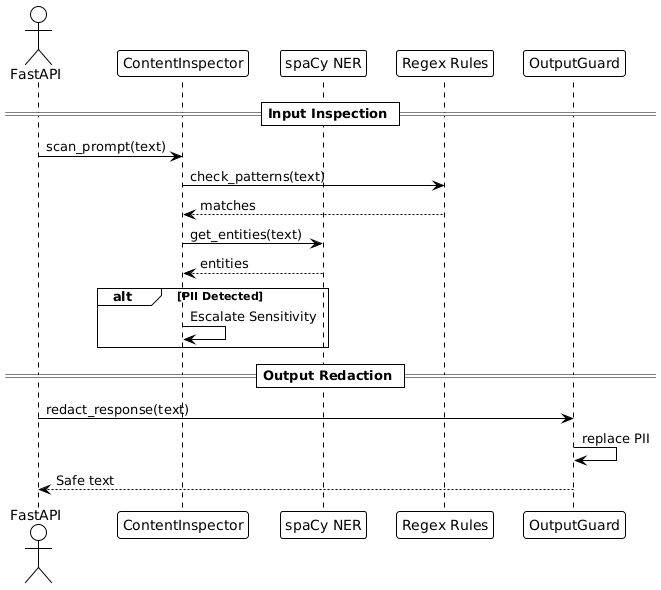
\includegraphics[width=0.85\textwidth]{images/sprint4_sequence.png}
    \caption{Prompt Injection Detection and PII Redaction Sequence}
    \label{fig:sprint4_sequence}
\end{figure}

The sequence diagram details the security hardening workflow:
\begin{enumerate}
    \item \textbf{Inbound Sanitization:} Incoming user prompts undergo strict sanitization against known jailbreak libraries and prompt injection signatures.
    \item \textbf{PII Detection:} The prompt is scanned for Personally Identifiable Information (PII) using Microsoft Presidio. If sensitive data (e.g., Credit Card, SSN) is detected, the request's sensitivity level is automatically escalated, potentially triggering stricter OPA governance rules.
    \item \textbf{Outbound Redaction:} As the AI generates the response stream, the \texttt{OutputGuardService} intercepts the text chunks in real-time. It scrubs the output, redacting any PII before the response is delivered to the end-user.
\end{enumerate}

\subsection{Showcase}
\label{subsec:sprint4_showcase}

The following figures showcase the advanced security hardening features of the platform.

\begin{figure}[H]
    \centering
    \includegraphics[width=0.85\textwidth]{images/prompt_injection_blocked.png}
    \caption{Proactive mitigation of a prompt injection attempt using the Microsoft Presidio-backed Security Service.}
    \label{fig:injection_block}
\end{figure}

\begin{figure}[H]
    \centering
    \includegraphics[width=0.85\textwidth]{images/frontend_pii_warning.png}
    \caption{Layer 1: Proactive client-side warning detecting personal data (phone numbers) before transmission.}
    \label{fig:frontend_pii_warning}
\end{figure}

\begin{figure}[H]
    \centering
    \includegraphics[width=0.85\textwidth]{images/pii_redaction.png}
    \caption{Layer 2: Real-time backend output sanitization: sensitive data redacted from the AI response stream.}
    \label{fig:pii_redaction}
\end{figure}

\begin{figure}[H]
    \centering
    \includegraphics[width=0.9\textwidth]{images/database_rls_proof.png}
    \caption{Technical proof of PostgreSQL Row-Level Security (RLS) enforcing deterministic tenant isolation at the database kernel level.}
    \label{fig:rls_proof}
\end{figure}


% ──────────────────────────────────────────────────────────────────
\section*{Conclusion}
\addcontentsline{toc}{section}{Conclusion}
% ──────────────────────────────────────────────────────────────────

In this chapter, we successfully implemented Release 2, significantly enhancing the platform's governance and security posture. Sprint 3 integrated OPA and Redis to enforce dynamic data policies and token quotas, providing administrators with granular control over AI consumption. Sprint 4 hardened the data layer with PostgreSQL Row-Level Security and established active threat mitigation guardrails, including prompt injection detection and real-time PII redaction. With a fully secured, governed, and orchestrated AI pipeline, the final release will focus on delivering complete operational visibility and deploying the platform for production use.
